%%
%% This is file `sigconf.tex',
%% generated with the docstrip utility.
%%
%% The original source files were:
%%
%% samples.dtx  (with options: `all,proceedings,sigconf')
%% 
%% IMPORTANT NOTICE:
%% 
%% For the copyright see the source file.
%% 
%% Any modified versions of this file must be renamed
%% with new filenames distinct from sigconf.tex.
%% 
%% For distribution of the original source see the terms
%% for copying and modification in the file samples.dtx.
%% 
%% This generated file may be distributed as long as the
%% original source files, as listed above, are part of the
%% same distribution. (The sources need not necessarily be
%% in the same archive or directory.)
%%
%%
%% Commands for TeXCount
%TC:macro \cite [option:text,text]
%TC:macro \citep [option:text,text]
%TC:macro \citet [option:text,text]
%TC:envir table 0 1
%TC:envir table* 0 1
%TC:envir tabular [ignore] word
%TC:envir displaymath 0 word
%TC:envir math 0 word
%TC:envir comment 0 0
%%
%% The first command in your LaTeX source must be the \documentclass
%% command.
%%
%% For submission and review of your manuscript please change the
%% command to \documentclass[manuscript, screen, review]{acmart}.
%%
%% When submitting camera ready or to TAPS, please change the command
%% to \documentclass[sigconf]{acmart} or whichever template is required
%% for your publication.
%%
%%
\documentclass[sigconf,screen,review]{acmart}

\usepackage{booktabs}
\usepackage{multirow}
\usepackage[table]{xcolor}
\definecolor{lightblue}{RGB}{235,245,255}
%%
%% \BibTeX command to typeset BibTeX logo in the docs
\AtBeginDocument{%
  \providecommand\BibTeX{{%
    Bib\TeX}}}

%% Rights management information.  This information is sent to you
%% when you complete the rights form.  These commands have SAMPLE
%% values in them; it is your responsibility as an author to replace
%% the commands and values with those provided to you when you
%% complete the rights form.
\setcopyright{none}
\settopmatter{printacmref=false, authorsperrow=3}
\renewcommand\footnotetextcopyrightpermission[1]{}

\acmConference[MM '26]{Proceedings of the 34th ACM International Conference on Multimedia}
{November 10--14, 2026}{Rio de Janeiro, Brazil}
\acmYear{2026}
\copyrightyear{2026}

%%
%% Submission ID.
%% Use this when submitting an article to a sponsored event. You'll
%% receive a unique submission ID from the organizers
%% of the event, and this ID should be used as the parameter to this command.
%%\acmSubmissionID{123-A56-BU3}

%%
%% For managing citations, it is recommended to use bibliography
%% files in BibTeX format.
%%
%% You can then either use BibTeX with the ACM-Reference-Format style,
%% or BibLaTeX with the acmnumeric or acmauthoryear sytles, that include
%% support for advanced citation of software artefact from the
%% biblatex-software package, also separately available on CTAN.
%%
%% Look at the sample-*-biblatex.tex files for templates showcasing
%% the biblatex styles.
%%
%%
%% The majority of ACM publications use numbered citations and
%% references.  The command \citestyle{authoryear} switches to the
%% "author year" style.
%%
%% If you are preparing content for an event
%% sponsored by ACM SIGGRAPH, you must use the "author year" style of
%% citations and references.
%% Uncommenting
%% the next command will enable that style.
%%\citestyle{acmauthoryear}


%%
%% end of the preamble, start of the body of the document source.
\begin{document}

%%
%% The "title" command has an optional parameter,
%% allowing the author to define a "short title" to be used in page headers.
\title{Semantics-Guided Feature Cutting and Batch Calibration for Low-Resource Multimodal Depression Assessment}

%%
%% The "author" command and its associated commands are used to define
%% the authors and their affiliations.
%% Of note is the shared affiliation of the first two authors, and the
%% "authornote" and "authornotemark" commands
%% used to denote shared contribution to the research.

\author{Zhengshuo Gong}
\affiliation{%
  \institution{School of Artificial Intelligence, Beijing University of Posts and Telecommunications}
  \city{Beijing}
  \country{China}
}
\email{gongzs729@bupt.edu.cn} % TODO: email not provided

\author{Zilu Zhang}
\affiliation{%
  \institution{School of Artificial Intelligence, Beijing University of Posts and Telecommunications}
  \city{Beijing}
  \country{China}
}
\email{zhangzilu@bupt.edu.cn}

\author{Yiming Ding}
\affiliation{%
  \institution{School of Artificial Intelligence, Beijing University of Posts and Telecommunications}
  \city{Beijing}
  \country{China}
}
\email{lololodym@bupt.edu.cn}

\author{Ziyi Guo}
\affiliation{%
  \institution{School of Artificial Intelligence, Beijing University of Posts and Telecommunications}
  \city{Beijing}
  \country{China}
}
\email{guoziyi2023@bupt.edu.cn}

\author{Yiming Jiang}
\affiliation{%
  \institution{School of Artificial Intelligence, Beijing University of Posts and Telecommunications}
  \city{Beijing}
  \country{China}
}
\email{jiang2005@bupt.edu.cn}

\author{Liang Tan}
\affiliation{%
  \institution{School of Artificial Intelligence, Beijing University of Posts and Telecommunications}
  \city{Beijing}
  \country{China}
}
\email{2023211884@bupt.cn} % TODO: email not provided

\author{Junyang Wu}
\affiliation{%
  \institution{School of Artificial Intelligence, Beijing University of Posts and Telecommunications}
  \city{Beijing}
  \country{China}
}
\email{wujunyang666@bupt.edu.cn}

\author{Yingying Zhou}
\affiliation{%
  \institution{School of Artificial Intelligence, Beijing University of Posts and Telecommunications}
  \city{Beijing}
  \country{China}
}
\email{yingyingzhou@bupt.edu.cn}

\author{Jingyao Xue}
\affiliation{%
  \institution{School of Artificial Intelligence, Beijing University of Posts and Telecommunications}
  \city{Beijing}
  \country{China}
}
\email{jingyaoxue@bupt.edu.cn}

\author{Yiming Gao}
\affiliation{%
  \institution{School of Artificial Intelligence, Beijing University of Posts and Telecommunications}
  \city{Beijing}
  \country{China}
}
\email{m15834150769@163.com}

\author{Yingming Gao}
\authornote{Corresponding authors.}
\affiliation{%
  \institution{School of Artificial Intelligence, Beijing University of Posts and Telecommunications}
  \city{Beijing}
  \country{China}
}
\email{yingming.gao@bupt.edu.cn}

\author{Ya Li}
\authornotemark[1]
\affiliation{%
  \institution{School of Artificial Intelligence, Beijing University of Posts and Telecommunications}
  \city{Beijing}
  \country{China}
}
\email{yli01@bupt.edu.cn}



%%
%% By default, the full list of authors will be used in the page
%% headers. Often, this list is too long, and will overlap
%% other information printed in the page headers. This command allows
%% the author to define a more concise list
%% of authors' names for this purpose.
\renewcommand{\shortauthors}{Gong et al.}
%%
%% The abstract is a short summary of the work to be presented in the
%% article.
\begin{abstract}
The MPDD-AVG challenge studies a valuable problem in affective computing and
mental-health assessment: estimating depression severity from multimodal
behavioural signals. The central difficulty is low-resource supervision: using
88 labelled Young-track training subjects, a system must select useful cues from
high-dimensional audio, video, gait, and personality data. We therefore build a
compact challenge system around three design principles: semantics-guided
feature cutting, shallow prediction, and metric-aware post-processing. The final
pipeline uses a gait--personality ordinal-ridge backbone, four OpenFace AU/gaze
temporal predictors, linear fusion, transductive batch-level moment alignment
for CCC, and a backbone-confirmed classification rule. We also report
exploratory routes across the Young modality settings: a G+P backbone, audio
and ASR studies, and the final A-V-G+P submission family. Local analyses
support compact IMU and OpenFace representations over several raw or
higher-dimensional alternatives, while preserved public-leaderboard checkpoints
document gains associated with facial AU/gaze dynamics, moment alignment, and
conservative classification. The final system achieves a public leaderboard
Score of \textbf{0.8745} on the MPDD-AVG 2026 Young track.
\end{abstract}

%%
%% CCS Concepts generated from the ACM CCS tool.
\begin{CCSXML}
<ccs2012>
<concept>
<concept_id>10010147.10010257</concept_id>
<concept_desc>Computing methodologies~Machine learning</concept_desc>
<concept_significance>500</concept_significance>
</concept>
<concept>
<concept_id>10010405.10010497</concept_id>
<concept_desc>Applied computing~Health informatics</concept_desc>
<concept_significance>300</concept_significance>
</concept>
</ccs2012>
\end{CCSXML}
\ccsdesc[500]{Computing methodologies~Machine learning}
\ccsdesc[300]{Applied computing~Health informatics}

\keywords{multimodal depression detection, low-resource learning, facial behaviour analysis, gait analysis, concordance calibration, PHQ-9 prediction}


%%
%% This command processes the author and affiliation and title
%% information and builds the first part of the formatted document.
\maketitle


\section{Introduction}

Depression is a major mental-health condition worldwide~\cite{who2017depression}. In clinical practice, screening tools such as PHQ-9 provide a structured way to measure symptom severity~\cite{kroenke2001phq}, while behavioural cues expressed through facial movement, gait, speech interaction, and personality-related traits can provide complementary information. The MPDD-AVG challenge offers a valuable benchmark for studying this problem under a unified multimodal protocol, requiring systems to estimate both continuous PHQ-9 severity and discrete depression labels.

A central difficulty of this setting is stable modelling under limited supervision. Depression-related multimodal data are inherently difficult and sensitive to collect, while raw behavioural descriptors can be high-dimensional and noisy. For the Young track, this means that simply increasing model capacity is not necessarily the best strategy. Instead, the system must control variance, retain interpretable signals, and make modelling choices that are robust under small-sample training.

The work reported here is organized around the Young modality settings rather
than only the best final score. The G+P setting motivates the stable
gait--personality backbone. Audio and ASR routes are retained as non-final
evidence about speech and language cues under limited supervision. The final
A-V-G+P submission family then combines the G+P backbone with compact visual
OpenFace predictors, while excluding speech branches that did not improve the
recorded development results.

Our final system follows this principle. We build a compact pipeline that first cuts each modality to semantically meaningful features, then combines several lightweight predictors. The main backbone, denoted \textsc{Orig}, uses the first three IMU acceleration channels together with Big-Five personality scores and fits an ordinal ridge regressor for PHQ-9 prediction. In parallel, the facial branch uses OpenFace AU and gaze streams only, summarised by four complementary temporal predictors: all-event statistics and facial change, event-3 state, cross-event drift, and spectral facial dynamics. The resulting PHQ-9 predictions are linearly fused, calibrated with transductive batch-level moment alignment for CCC, and converted into binary and ternary labels with a backbone-confirmed rule.

\noindent\textbf{Contributions.}
This paper makes four contributions. (1) We present a fully specified
low-resource system for MPDD-AVG Young, combining gait--personality modelling,
OpenFace temporal predictors, batch calibration, and rule-based label
derivation. (2) We organize the system history across the Young modality
settings: G+P for the backbone, audio/ASR and deep sequence models as non-final
explorations, and A-V-G+P for the final multimodal submission family. (3) We
provide local evidence for semantics-guided feature cutting, where compact IMU
and OpenFace representations outperform several raw or higher-dimensional
alternatives in recorded analyses. (4) We separate controlled local design
evidence from public-leaderboard development feedback, including the
transductive calibration and final threshold choices. The submitted system
achieves a public leaderboard Score of \textbf{0.8745} on the MPDD-AVG 2026
Young track.
\section{Related Work}

\subsection{Multimodal Depression Detection}
Automatic depression detection has been widely studied with interview, speech,
facial, language, and physiological or behavioural signals. This fits the
broader multimodal machine-learning setting, where complementary modalities must
be represented, aligned, fused, and regularized under limited supervision
~\cite{baltrusaitis2019multimodal}. Early benchmark resources such as DAIC-WoZ
provided structured human--computer interview data for distress
analysis~\cite{gratch2014daic}, while AVEC standardised audio-visual depression
and affect recognition evaluation protocols~\cite{ringeval2019avec}. More
recent datasets extend this direction to naturalistic or clinical multimodal
settings, including D-Vlog~\cite{yoon2022dvlog}, EATD~\cite{shen2022eatd}, and
MODMA~\cite{cai2022modma}. The MPDD challenge introduces personality-aware
depression detection and provides a unified benchmark for multimodal PHQ-9
estimation~\cite{fu2025mpdd}. Our work follows this multimodal line, but
focuses on a compact system design rather than high-capacity end-to-end fusion.

\subsection{Personality and Facial Behaviour Modelling}
Personality information is relevant to depression assessment because individual
traits can affect both symptom expression and behavioural responses. We use the
Big-Five trait representation, a standard taxonomy for personality
measurement~\cite{john1999bigfive}. Prior MPDD systems have therefore explored
personality-enhanced multimodal fusion~\cite{wang2025personality},
hypergraph-based personality-aware modelling~\cite{fu2026p3hf}, and comparative
machine-learning or language-model approaches~\cite{hong2025exploring}. Facial
behaviour is another commonly used signal in depression detection, because
reduced expressiveness, gaze changes, and action-unit dynamics can reflect
affective and psychomotor states. AU terminology follows the Facial Action
Coding System~\cite{ekman1978facs}. We use OpenFace~\cite{baltrusaitis2018openface}
to extract interpretable facial streams, but retain only AU and gaze features
rather than using the full raw descriptor. This choice connects the facial
branch to explicit behavioural cues and keeps the representation compact.

\subsection{Low-Resource and Metric-Aware Modelling}
Mental-health datasets are naturally difficult to scale because of privacy, annotation cost, and participant recruitment constraints. Under such conditions, high-dimensional representations can introduce large estimation variance, making feature selection and task-driven dimensionality reduction important. Our system uses this low-resource bias throughout: IMU streams are reduced to acceleration-based gait statistics, personality descriptions are reduced to Big-Five scores, and OpenFace outputs are reduced to AU/gaze streams. We nevertheless explored speech representations such as openSMILE descriptors~\cite{eyben2013opensmile} and wav2vec2 embeddings~\cite{baevski2020wav2vec}; these routes are reported as negative evidence rather than final-system components. For the facial predictors, we additionally use mixup~\cite{zhang2018mixup} and seed averaging to reduce instability.

The MPDD-AVG score also encourages metric-aware modelling. Continuous PHQ-9 prediction is evaluated with the concordance correlation coefficient (CCC), which penalises not only rank disagreement but also mean and variance mismatch~\cite{lin1989ccc}. Discrete labels are assessed with classification and agreement metrics, including Cohen's kappa~\cite{cohen1960kappa}. These metrics differ from ordinary regression losses and motivate our transductive moment-alignment and rule-based classification steps. The backbone further treats PHQ-9 as an ordered severity target through ordinal ridge regression, implemented with the \texttt{mord} ordinal regression package~\cite{mord}. These choices allow the final system to remain simple while matching the structure of the official evaluation.
\section{Methodology}
\label{sec:method}

\begin{figure*}[t]
  \centering
  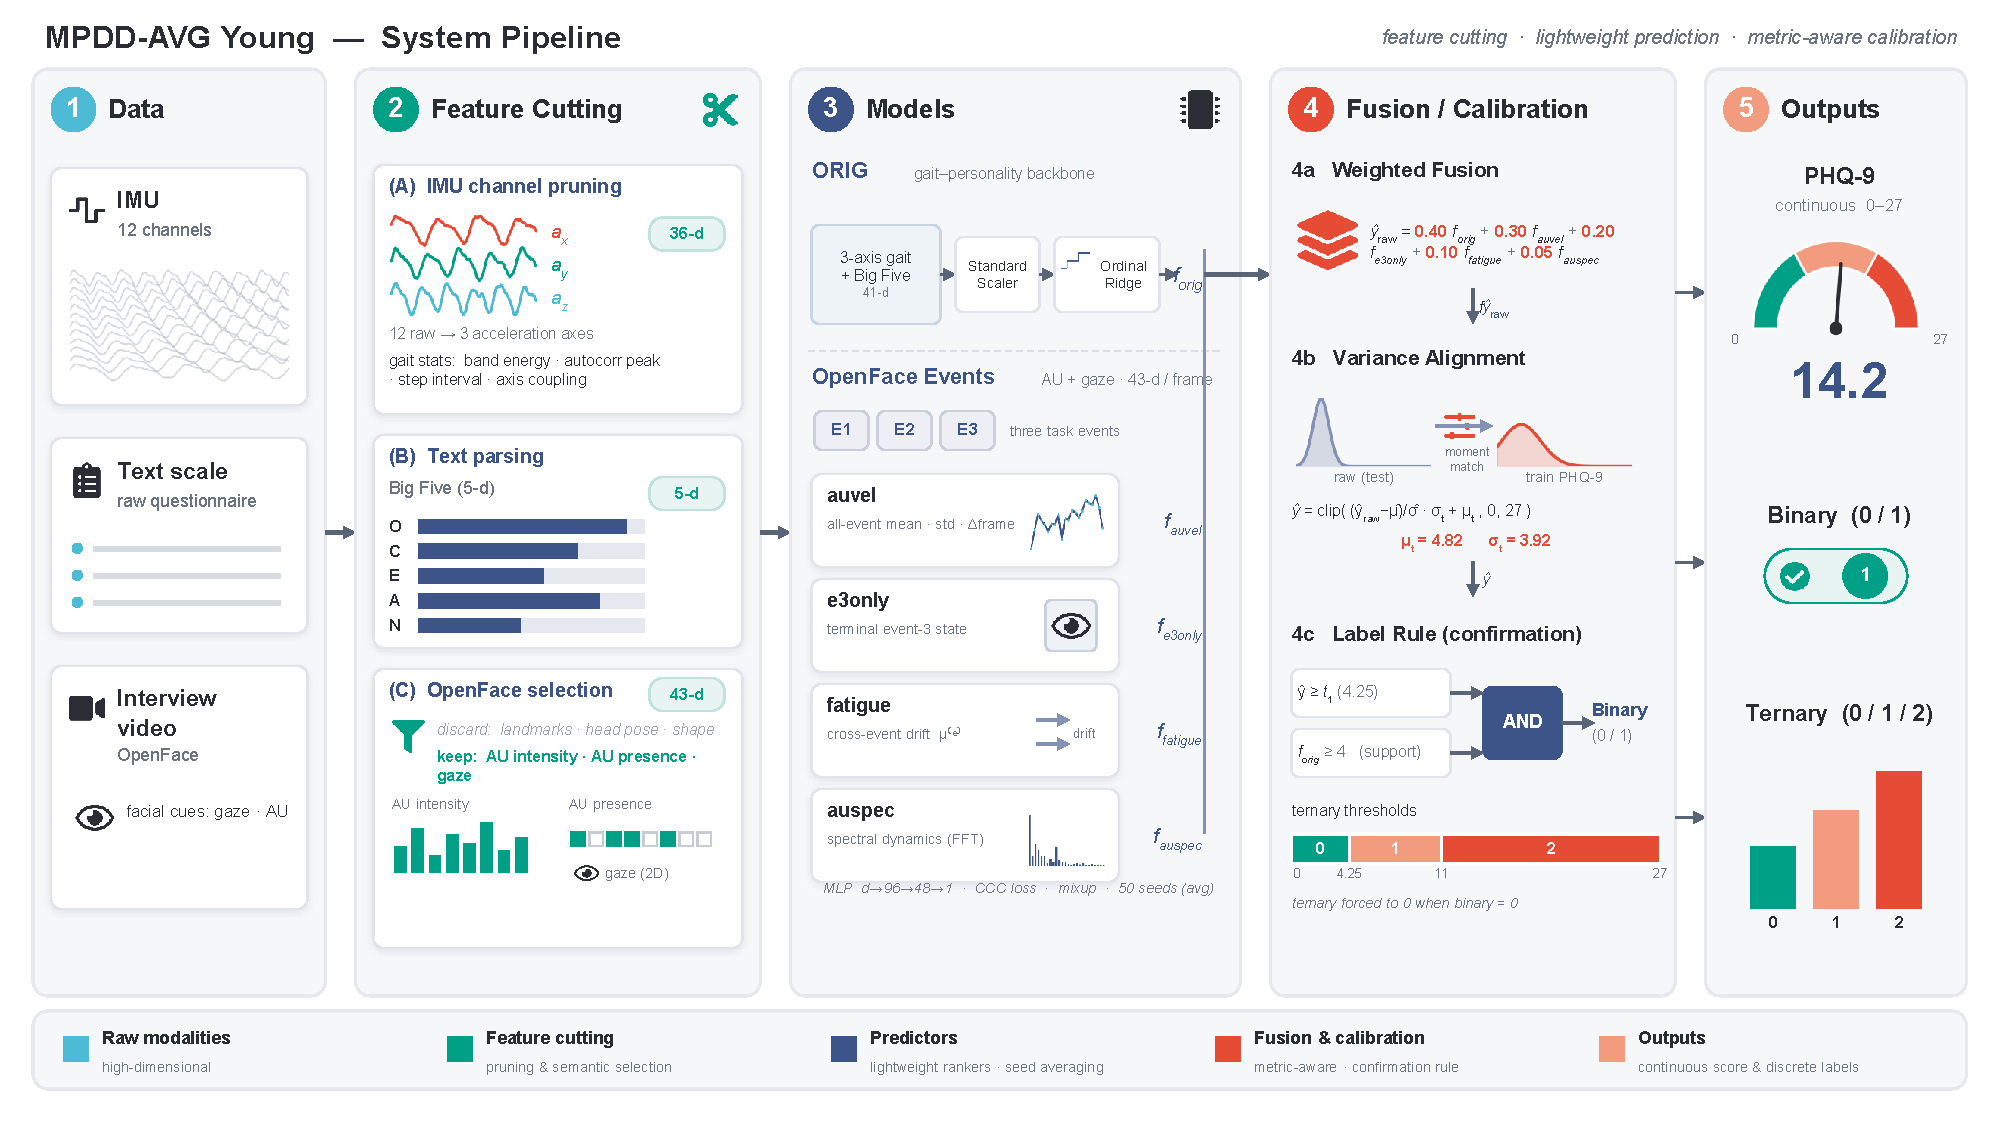
\includegraphics[width=\textwidth]{fig/MPDD-AVG_architecture_export.pdf}
  \Description{System pipeline diagram for MPDD-AVG Young. The figure shows
  raw IMU, text-scale, and interview-video inputs, feature cutting into
  compact IMU, Big-Five, and OpenFace AU/gaze cues, lightweight ORIG and
  OpenFace predictors, weighted fusion, batch-level moment alignment, label-rule
  confirmation, and PHQ-9, binary, and ternary outputs.}
  \caption{Overview of the submitted MPDD-AVG Young system. The pipeline first
  cuts raw IMU, personality-scale text, and OpenFace streams into compact
  behavioural cues, then applies an ordinal gait--personality backbone and four
  OpenFace temporal predictors. The five continuous predictions are linearly
  fused, batch-calibrated for CCC, and converted into binary and ternary labels
  with backbone confirmation.}
  \label{fig:architecture}
\end{figure*}

\subsection{Feature Cutting}
\label{sec:method-cutting}

Figure~\ref{fig:architecture} summarizes the submitted system. It is designed
around a simple observation: in this task, the number of labelled training
subjects is much smaller than the dimensionality of many raw behavioural
descriptors. Directly fitting high-dimensional video or sensor descriptors can
therefore produce unstable predictors whose apparent training signal is
dominated by sample-specific correlations. We use feature cutting as the first
modelling step: each retained modality is reduced to a small set of semantically
interpretable signals before any supervised model is trained.

The final system keeps three information sources. First, from the IMU stream we
retain only the first three channels, corresponding to the acceleration axes
$(a_x,a_y,a_z)$. These channels directly describe gait rhythm, movement
intensity, and body-motion periodicity. The remaining IMU channels are not
treated as physically meaningless, but they substantially increase the
feature-to-sample ratio and were less reliable in our dimension-selection
experiments. Second, from the personality descriptions we parse only the five
Big-Five scores. This converts free-form text into a compact personality vector
and avoids introducing a high-dimensional language embedding into the final
model. Third, from OpenFace we discard landmarks, head pose, and shape
parameters, and keep only facial behaviour streams: gaze, action-unit (AU)
intensities, and AU presence indicators. This gives an interpretable
43-dimensional per-frame facial signal rather than a raw OpenFace descriptor.

This cutting step is not a post-hoc compression of a large trained model. It is
part of the modelling assumption: semantics-guided feature selection and
temporal summarisation are used to control estimation variance under limited
supervision. The later predictors are deliberately shallow relative to
sequence-level end-to-end alternatives: an ordinal ridge backbone for
IMU/personality and two-hidden-layer MLPs for facial temporal summaries. The
goal is to preserve behavioural cues relevant to depression severity---gait
dynamics, personality traits, gaze, and facial action patterns---without fitting
the full raw descriptors directly.

\subsection{\textsc{Orig} Backbone}
\label{sec:method-orig}

The backbone, denoted \textsc{Orig}, uses the acceleration channels and Big-Five
personality scores. Let $s$ be one acceleration axis sampled at $f_s=50$ Hz. For
each axis, we extract band-energy, variation, periodicity, and peak-interval
features. We first apply fourth-order Butterworth band-pass filters with
zero-phase \texttt{filtfilt} filtering to obtain
three frequency components: a gait band ($0.5$--$1.5$ Hz), a locomotion band
($1.5$--$3$ Hz), and a high-frequency band ($3$--$10$ Hz). For band $b_k$, the
relative energy is
\begin{equation}
r_k =
\frac{\sum_t s_{b_k}(t)^2}
{\sum_t s(t)^2+\epsilon},
\qquad k\in\{1,2,3\}.
\label{eq:imu-energy}
\end{equation}
For the two lower-frequency bands, we also compute the coefficient-of-variation
statistic used in the submitted code,
\begin{equation}
\mathrm{CV}_k =
\frac{\mathrm{std}(s_{b_k})}
{|\mathrm{mean}(s_{b_k})|+\epsilon}.
\label{eq:imu-cv}
\end{equation}
with $\epsilon=10^{-8}$. Because a band-pass output can have a small mean, this
quantity should be interpreted as a code-level descriptive statistic rather than
a physically calibrated variability measure; the downstream scaler standardizes
all IMU features before regression.

To capture gait periodicity, we compute the normalized autocorrelation
\begin{equation}
R(\tau)=
\frac{\sum_t (s_t-\bar{s})(s_{t+\tau}-\bar{s})}
{\sum_t (s_t-\bar{s})^2},
\label{eq:imu-autocorr}
\end{equation}
and record the first peak in the lag range $\tau\in[1,100)$ whose height is at
least $0.3$, together with the corresponding period $\tau/f_s$. We further
detect signal peaks with a minimum distance of $f_s/4$ and prominence $0.5$,
then compute the mean, standard deviation, and coefficient of variation of
inter-peak intervals. Thus each acceleration axis contributes 10 features:
three band-energy ratios, two band CVs, autocorrelation peak height, dominant
period, and three peak-interval statistics.

Across the three axes we add six aggregate features: the pairwise correlations
$\rho_{xy}$, $\rho_{xz}$, $\rho_{yz}$ and the mean, standard deviation, and
coefficient of variation of acceleration magnitude
\begin{equation}
\|a\|=\sqrt{a_x^2+a_y^2+a_z^2}.
\label{eq:accel-mag}
\end{equation}
The IMU representation is therefore $3\times10+6=36$ dimensional. We concatenate
five parsed Big-Five scores, yielding a 41-dimensional input vector for the
backbone.

All backbone features are standardized with training-set statistics:
\begin{equation}
\tilde{x}_{ij} =
\frac{x_{ij}-\mu_j}{\sigma_j+\epsilon},
\qquad
\mu_j,\sigma_j\ \text{estimated on the training split only}.
\label{eq:standardize}
\end{equation}
The same scaler is then applied to the test subjects. For the target, the
training PHQ-9 values are first mapped to their observed ordinal indices. If
$\mathcal{Y}=\{v_1<\cdots<v_K\}$ is the sorted set of PHQ-9 scores appearing in
the training labels, then a score $v_k$ is encoded as class index $k-1$. We fit
an ordinal ridge regressor~\cite{mord} with $\alpha=1.0$ to predict this ordered
index:
\begin{equation}
f_{\textsc{orig}}:
\quad
\texttt{StandardScaler}
\rightarrow
\texttt{OrdinalRidge}(\alpha=1.0).
\label{eq:orig-model}
\end{equation}
The predicted ordinal index is rounded internally by the model and mapped back
to the corresponding PHQ-9 value in $\mathcal{Y}$. This output is used both as a
continuous PHQ-9 predictor and as a confirmation signal in the final
classification rule.

\subsection{OpenFace Block}
\label{sec:method-openface}

OpenFace is used as an interpretable facial behaviour extractor. In the
preprocessed OpenFace arrays, the first column is the frame index; after
removing it, the facial block keeps 43 columns:
\begin{equation}
8\ \text{gaze} \;+\; 17\ \text{AU intensities}
\;+\; 18\ \text{AU presence indicators}.
\end{equation}
For event $e\in\{1,2,3\}$, let
$X^{(e)}\in\mathbb{R}^{T_e\times43}$ denote the selected OpenFace sequence. We
build four complementary summaries from this sequence, each trained as an
independent PHQ-9 predictor.

\paragraph{\textsc{auvel}.}
The \textsc{auvel} view summarizes all three events. For each event, it
concatenates the per-channel temporal mean, temporal standard deviation, and
mean absolute frame-to-frame change:
\begin{equation}
\phi^{(e)}_{\text{auvel}} =
\left[
\mathrm{mean}_t X^{(e)},\;
\mathrm{std}_t X^{(e)},\;
\frac{1}{T_e-1}\sum_{t=1}^{T_e-1}
\left|X^{(e)}_{t+1}-X^{(e)}_t\right|
\right].
\label{eq:auvel}
\end{equation}
Each event contributes $3\times43=129$ features, and concatenating the three
events gives a 387-dimensional vector. The frame-change term is a discrete
facial-motion proxy rather than a calibrated physical velocity.

\paragraph{\textsc{e3only}.}
The \textsc{e3only} view uses the same mean, standard deviation, and
frame-change statistics, but only from event 3. It is 129-dimensional and is
intended to emphasize the final-task facial state, which may reflect accumulated
task effects.

\paragraph{Cross-event drift (\textsc{fatigue}).}
The \textsc{fatigue} code path represents cross-event drift. Let
$\mu^{(e)}=\mathrm{mean}_t X^{(e)}$. We encode
\begin{equation}
\phi_{\text{fatigue}} =
\left[
\mu^{(2)}-\mu^{(1)},\;
\mu^{(3)}-\mu^{(2)},\;
\mu^{(3)}-\mu^{(1)}
\right],
\label{eq:fatigue}
\end{equation}
which gives $3\times43=129$ features. This block captures whether expression,
gaze, or AU activation changes systematically across the session.

\paragraph{\textsc{auspec}.}
The \textsc{auspec} view describes spectral facial dynamics. For each event, the
43 selected OpenFace channels are mean-centered and transformed with a real FFT.
Let $A_f$ be the magnitude spectrum for one channel. The frequency bins are
split into low, middle, and high thirds. Following the submitted implementation,
we compute three normalized spectral magnitude ratios, spectral entropy, and
normalized dominant frequency:
\begin{equation}
p_f=\frac{A_f}{\sum_{f'} A_{f'}+\epsilon},
\label{eq:auspec}
\end{equation}
with entropy and normalized dominant frequency
\begin{equation}
H=-\sum_f p_f\log(p_f+\epsilon),
\qquad
d=\frac{\arg\max_f A_f}{F+\epsilon}.
\label{eq:auspec-extra}
\end{equation}
Together with the three magnitude ratios, this gives five spectral statistics
per channel, or $5\times43=215$ features per event. Concatenating the three
events gives a 645-dimensional vector.

\paragraph{CCC-loss MLP training.}
Each facial view is standardized with a training-only \texttt{StandardScaler}
and trained using the same two-hidden-layer MLP:
\begin{equation}
d \rightarrow 96 \rightarrow 48 \rightarrow 1,
\label{eq:mlp-arch}
\end{equation}
with GELU activations and dropout rate $0.3$. Since the leaderboard score
contains CCC, the loss directly optimizes concordance with a small MSE term:
\begin{equation}
\mathcal{L}
=
\left(1-\mathrm{CCC}(y_m,\hat{y}_m)\right)
+0.1\,\mathrm{MSE}(y_m,\hat{y}_m).
\label{eq:ccc-loss}
\end{equation}
The CCC term is computed as
\begin{equation}
\mathrm{CCC}(y,\hat{y})
=
\frac{2\,\mathrm{cov}(y,\hat{y})}
{\mathrm{var}(y)+\mathrm{var}(\hat{y})+
(\mathrm{mean}(y)-\mathrm{mean}(\hat{y}))^2}.
\label{eq:ccc}
\end{equation}

Training uses mixup~\cite{zhang2018mixup}. At each epoch, 2000 synthetic samples
are drawn by sampling two training subjects $a,b$ and a mixing coefficient
$\lambda\sim\mathrm{Beta}(0.4,0.4)$:
\begin{equation}
X_m=\lambda X_a+(1-\lambda)X_b,
\qquad
y_m=\lambda y_a+(1-\lambda)y_b.
\label{eq:mixup}
\end{equation}
One full-batch AdamW~\cite{loshchilov2019decoupled} update is then taken on these 2000 mixed samples. Each MLP
is trained for 400 epochs with learning rate $10^{-3}$, weight decay $10^{-3}$,
and gradient clipping at 1.0. Every 20 epochs, CCC is evaluated on the original
training subjects, and the best checkpoint is retained. To reduce seed
variance, each facial view is trained with 50 random seeds and the test
predictions are averaged, producing
$f_{\text{auvel}}$, $f_{\text{e3only}}$, $f_{\text{fatigue}}$, and
$f_{\text{auspec}}$.

\subsection{Fusion, Batch-Level Moment Alignment, and Classification}
\label{sec:method-fusion}

The final continuous PHQ-9 prediction is a fixed linear blend of the backbone
and four OpenFace predictors:
\begin{equation}
\hat{y}_{\mathrm{raw}} =
0.40 f_{\textsc{orig}}
+0.30 f_{\text{auvel}}
+0.20 f_{\text{e3only}}
+0.10 f_{\text{fatigue}}
+0.05 f_{\text{auspec}}.
\label{eq:fusion}
\end{equation}
The weights are not constrained to sum to one, because the next step applies a
global affine rescaling. They specify the relative contribution of the backbone
and each facial view.

Small-sample regressors often shrink predictions toward the training mean. This
is especially harmful for CCC, whose denominator penalizes not only errors in
ranking but also mismatch in mean and variance, as shown in
Eq.~\ref{eq:ccc}. We therefore apply a transductive, batch-level moment
alignment step that maps the blended public-test predictions to target PHQ-9
moments:
\begin{equation}
\hat{y}
=
\mathrm{clip}\left(
\frac{
\hat{y}_{\mathrm{raw}}-\overline{\hat{y}}_{\mathrm{raw}}
}
{\mathrm{std}(\hat{y}_{\mathrm{raw}})+\epsilon}
\sigma_t+\mu_t,\;
0,\;27
\right).
\label{eq:variance-align}
\end{equation}
Here $\overline{\hat{y}}_{\mathrm{raw}}$ and
$\mathrm{std}(\hat{y}_{\mathrm{raw}})$ are computed over the test batch, while
the target moments are fixed to $\mu_t=4.82$ and $\sigma_t=3.92$ in the
submitted configuration. This operation uses no individual test labels, but it
does use the unlabelled test-batch distribution; it is therefore a transductive
batch-level calibration step rather than a single-subject online calibration
procedure. Before clipping, the alignment preserves the rank order of the
blended predictions and corrects their location and scale. The clipping simply
enforces the valid PHQ-9 range $[0,27]$.

The official task also evaluates binary and ternary labels. Instead of training
a separate classifier, we derive labels from the calibrated PHQ-9 prediction and
use the \textsc{Orig} backbone as a confirmation branch. The binary prediction
is
\begin{equation}
\hat{y}_2 =
\mathbb{1}\left[
\hat{y}\ge t_1
\;\wedge\;
f_{\textsc{orig}}\ge 4
\right].
\label{eq:binary-rule}
\end{equation}
The ternary prediction is first thresholded from the calibrated score,
\begin{equation}
\hat{y}_3 =
\begin{cases}
0, & \hat{y}<t_1,\\
1, & t_1\le \hat{y}<t_2,\\
2, & \hat{y}\ge t_2,
\end{cases}
\label{eq:ternary-rule}
\end{equation}
and is then forced to zero whenever $\hat{y}_2=0$. This conjunctive rule reduces
false positives whose ensemble score is driven mainly by the facial predictors but
is not supported by the gait-personality backbone. In the final submitted
configuration, we use $t_1=4.25$ and $t_2=11.0$, selected from public
leaderboard feedback.

\section{Experiments}
\label{sec:experiments}

\subsection{Experimental Protocol}
\label{sec:exp-protocol}

The experiments are organized around the design choices of the final system and
the Young modality settings. The G+P setting is represented by the
IMU--personality \textsc{Orig} backbone. Audio, ASR, and deep sequence trials
are reported as non-final speech/video explorations. The final submitted system
belongs to the A-V-G+P family, but its retained inputs are IMU acceleration,
Big-Five scores, and OpenFace AU/gaze streams because the speech branches did
not improve the recorded development results.

We report three types of empirical evidence. \textbf{Local design analyses}
justify feature-cutting decisions and are not treated as official challenge
scores. \textbf{Public-leaderboard checkpoints} document the cumulative
development trajectory of the submitted system. \textbf{Non-final explorations}
record speech and deep-sequence routes that were considered but excluded from
the final ensemble. The official score combines the binary classification term,
the PHQ-9 concordance term, and the ternary classification term:
\begin{equation}
\mathrm{Score}
=
\frac{1}{3}
\left(
\mathrm{F1}
+\mathrm{CCC}
+\mathrm{Kappa}
\right).
\label{eq:official-score}
\end{equation}
All leaderboard results are from submissions to the MPDD-AVG Young public split.
No individual test labels were available; however, aggregate public-leaderboard
feedback was used to select the final decision thresholds. We therefore treat
the public split as a development benchmark rather than an unbiased held-out
test set.

\subsection{Effect of Compact Feature Design}
\label{sec:exp-cutting}

We first examine whether the compact feature design in Sec.~\ref{sec:method} is
empirically justified. Table~\ref{tab:feature_cutting_binary} reports local
evidence for two final-system design choices: retaining only the acceleration
channels from IMU and using compact OpenFace representations rather than raw
high-dimensional descriptors.

For IMU, we isolate the channel-selection question by using IMU-only
hand-crafted features and leave-one-out validation on the Young training set.
Across the compared Ridge models, the 3-channel acceleration setting gives the
lowest PHQ-9 MAE. Adding channels increases the feature dimension from 36 to
78, 129, and 189, but does not reduce the error. This supports the use of the
first three acceleration channels as the IMU part of \textsc{Orig}. For
OpenFace, raw 710-dimensional features with a linear classifier perform at
chance level in the local binary analysis, while PCA5 improves the binary
accuracy to 0.682. A separate semantic subset analysis further shows that
AU/gaze statistics outperform the complete semantic OpenFace feature set under
the same direct binary evaluation. These results support the final facial
design, which keeps AU/gaze streams and summarizes them through event-level,
temporal-change, and spectral descriptors.

\begin{table}[!t]
\centering
\caption{Local evidence for compact feature design. Panel A isolates IMU
channel pruning with Young-train LOO Ridge regression; Panel B summarizes
OpenFace dimensionality reduction and semantic feature selection with local
binary classification. These numbers are design evidence, not official
CodaBench scores.}
\label{tab:feature_cutting_binary}
\small
\setlength{\tabcolsep}{5pt}
\renewcommand{\arraystretch}{1.08}
\begin{tabular}{lccc}
\toprule
\multicolumn{4}{l}{\textbf{A. IMU channel pruning (LOO Ridge, MAE $\downarrow$)}} \\
\midrule
\textbf{Input channels} & \textbf{Dim} & \textbf{MAE} & \textbf{vs. 3-axis} \\
\midrule
3 accel. channels & 36  & \textbf{3.444} & -- \\
6 channels        & 78  & 5.563          & +2.119 \\
9 channels        & 129 & 4.945          & +1.501 \\
12 channels       & 189 & 4.765          & +1.321 \\
\midrule
\multicolumn{4}{l}{\textbf{B. OpenFace cutting (local LR, binary accuracy $\uparrow$)}} \\
\midrule
\textbf{Comparison} & \textbf{Setting} & \textbf{Dim} & \textbf{Acc.} \\
\midrule
PCA compression & Raw descriptor    & 710 & 0.500 \\
PCA compression & PCA5              & 5   & \textbf{0.682} \\
Semantic subset & All semantic stats & 479 & 0.682 \\
Semantic subset & AU+gaze stats      & 399 & \textbf{0.727} \\

\bottomrule
\end{tabular}
\end{table}


These analyses should be interpreted conservatively. They do not imply that
lower dimensionality is always better; rather, they indicate that semantically
constrained reductions are more reliable than broad high-dimensional inputs in
this limited-sample setting.

\subsection{Cumulative Contribution of Final Components}
\label{sec:exp-components}

Table~\ref{tab:stepwise_components} summarizes the preserved cumulative
development checkpoints of the final system family on the public leaderboard.
The table is not a strict leave-one-component-out ablation, because not every
historical intermediate submission was preserved as an independent clean
script. It is therefore used as historical public-leaderboard trajectory
evidence rather than as a fully controlled ablation study.

\begin{table}[!t]
\centering
\caption{Historical public-leaderboard trajectory of the final system family.
The rows are preserved cumulative development checkpoints, not strict
leave-one-component-out ablations.}
\label{tab:stepwise_components}
\footnotesize
\setlength{\tabcolsep}{2.5pt}
\renewcommand{\arraystretch}{1.05}
\begin{tabular}{p{0.35\columnwidth}rrrr}
\toprule
\textbf{Checkpoint} & \textbf{Score} & \textbf{F1} & \textbf{CCC} & \textbf{Kappa} \\
\midrule
\textsc{Orig} backbone       & 0.6701 & 0.7972 & 0.5083 & 0.7048 \\
+ OpenFace AU/gaze           & 0.7063 & 0.7972 & 0.6170 & 0.7048 \\
+ Frame-change / multi-view  & 0.7178 & 0.7972 & 0.6515 & 0.7048 \\
+ Batch moment alignment     & 0.7931 & 0.7972 & 0.8772 & 0.7048 \\
+ AND classification rule    & 0.8347 & 0.8361 & 0.8772 & 0.8012 \\
+ Final thresholding         & \textbf{0.8745} & -- & 0.8772 & -- \\
\bottomrule
\end{tabular}
\end{table}


The progression identifies changes that were associated with the main
leaderboard increases. The \textsc{Orig} backbone provides a low-dimensional
baseline. Adding OpenFace AU/gaze features is associated with an increase in the
continuous PHQ-9 component, with CCC moving from 0.5083 to 0.6170. Adding
frame-change and multi-view facial predictors further moves CCC to 0.6515. The
largest single change is batch-level moment alignment: after matching the
prediction distribution to target PHQ-9 moments, CCC reaches 0.8772 and the
overall score reaches 0.7931. Finally, the AND classification rule improves the
discrete classification terms, raising F1 from 0.7972 to 0.8361 and Kappa from
0.7048 to 0.8012 while leaving the calibrated CCC unchanged in the preserved
checkpoint. The final submitted threshold configuration has a retained public
Score of 0.8745 and CCC of 0.8772; its separate F1 and Kappa values were not
preserved in the local result package.

\subsection{Explored Routes Outside the Final Ensemble}
\label{sec:exp-negative}

We also evaluated routes that correspond to the broader available modalities but
did not enter the final submission. Speech features included MFCC/openSMILE
descriptors, wav2vec2 embeddings, temporal GRU models, and an ASR-based PHQ-9
symptom-prior route. These experiments were useful for model selection but were
not competitive with the compact gait--personality and OpenFace pipeline: the
GRU sequence models reached binary F1 values of 0.5856 for openSMILE and 0.5227
for wav2vec2 in recorded local experiments, and the standalone ASR route reached
a public Score of 0.457751. We therefore report these audio and language routes
as negative evidence under the 88-subject training regime, not as final-system
components.

\subsection{Final Submission and Reproducibility}
\label{sec:exp-final}

The final submitted system uses three sources of information: IMU acceleration
features, Big-Five personality scores, and OpenFace AU/gaze streams. The
consolidated pipeline contains the \textsc{Orig} backbone, the four facial
predictors, linear fusion, batch-level moment alignment, and submission-file
generation. It is preserved in the reproduction package through a single
pipeline entry script, the \textsc{Orig} builder, and the four OpenFace predictor
builders, with standard scaling and linear models implemented through
scikit-learn~\cite{pedregosa2011scikit}. The final submitted configuration
obtains a public leaderboard score of \textbf{0.8745}.



\section{Limitations and Conclusion}
\label{sec:conclusion}

We presented a compact multimodal system for the MPDD-AVG 2026 Young track.
The system combines an IMU--personality ordinal backbone with four OpenFace
AU/gaze temporal predictors, then applies linear fusion, transductive
batch-level moment alignment, and a backbone-confirmed classification rule. The
evidence supports the central design principle that, under limited supervision,
semantically selected compact features and metric-aware post-processing can be
competitive with broader high-dimensional modelling.

Several limitations should be made explicit. The public leaderboard was used as
development feedback for decision thresholds, so the reported public score is
not an unbiased estimate of hidden-test performance. The moment-alignment step
uses the unlabelled test-batch distribution and is therefore not a single-subject
online calibration procedure. The system is a challenge submission for
depression-severity estimation, not a clinical diagnostic tool, and its behaviour
across institutions, devices, and populations remains unverified. Within these
conditions, the final submitted system achieves a public leaderboard Score of
\textbf{0.8745}.

\bibliographystyle{ACM-Reference-Format}
\bibliography{references}

\end{document}
\endinput
%%
%% End of file `sigconf.tex'.



